\documentclass[9pt, french, brown]{beamer}

\usetheme{Rochester} 
\setbeamertemplate{footline}[frame number]
\setbeamertemplate{navigation symbols}{}
\hypersetup{colorlinks,linkcolor=blue,urlcolor=blue}

\usepackage[french]{babel}
\usepackage[utf8]{inputenc}
\usepackage[T1]{fontenc}

\usepackage{graphics}
\usepackage{multirow}
\usepackage{color, colortbl}
\usepackage[misc]{ifsym} % pour le symbole de l'enveloppe
\usepackage{fancybox} % pour encadrement test

\setbeamertemplate{itemize subitem}[triangle]
\definecolor{vert}{rgb}{0,0.4,0}
\newcommand{\mytitle}[1]{{\color{brown}#1 \\~\\}}


%~~~~~~~~~~~~~~~~~~~~~~~~~~~~~~~~~~~~~~~~~~~~~~~~~~~~~~~~~~~~~~~~~~~~~~~~~~~~~~~
\title{Python}
\subtitle{Interface graphique avec Qt}
\author{D.~DUBOIS\let\thefootnote\relax\footnotetext{ \href{mailto:dimitri.dubois@umontpellier.fr}{\Letter ~dimitri.dubois@umontpellier..fr}}}
\institute{{\normalsize Diplôme Universitaire\\~\\CFI2L}\\~\\~\\Faculté d'Economie de Montpellier\\~\\~\\

\includegraphics[width=0.2 \textwidth]{img/pyqt}}
\date{}
%~~~~~~~~~~~~~~~~~~~~~~~~~~~~~~~~~~~~~~~~~~~~~~~~~~~~~~~~~~~~~~~~~~~~~~~~~~~~~~~


\begin{document}

\begin{frame}[plain]
\titlepage
\end{frame}

\begin{frame}{Plan}
\tableofcontents[sections=1-2]
\end{frame}

\begin{frame}{Plan}
\tableofcontents[sections=3-]
\end{frame}

%===============================================================================
\begin{frame}{Introduction}
\mytitle{Qt}
\begin{itemize}
\item Bibliothèque logicielle offrant des composants d\rq{}interface graphique (widgets)
\item Développée par Trolltech, depuis 1991
\item Développée en C++
\item Sous licence LGPL ou propriétaire
\item Utilisé par Skype, Google, Boeing, Adobe, la NASA \ldots
\item Actuellement la version 5 (Qt5)
\end{itemize}
~\\
\mytitle{Autres bibliothèques graphiques}
\begin{itemize}
\item framework .NET (windows). Utilisable avec C++ et c\#
\item Cocoa (Mac OS). Utilisable avec Objective C.
\item GTK+ (Linux gnome).
\item Aussi wxWidgets, FLTK
\end{itemize}
\end{frame}

\begin{frame}{Introduction}{Qt}
\mytitle{De nombreux modules}
\begin{itemize}
\item QtCore: la boucle événementielle, le mécanisme des signaux/slots, les threads \ldots
\item QtWidgets: éléments graphiques
\item QtWebKit: pour implémenter un navigateur web
\item QtMultimedia: pour le multimédia
\item \ldots
\end{itemize}
Liste: \url{http://doc.qt.io/qt-5/modules-cpp.html}
\end{frame}

\begin{frame}{Introduction}{Qt - les plus}
\begin{itemize}
\item Multiplateforme
\item Gratuit (licence LGPL)
\item Simple d\rq{}utilisation
\item Propose des outils comme  Qt Designer pour la création des interfaces graphiques ou Qt Linguist pour l\rq{}internationalisation de l\rq{}application
\item Utilise le look and feel natif du système
\end{itemize}
\end{frame}

\begin{frame}{Introduction}{Qt - documentation}
\mytitle{Beaucoup de documentation}
\begin{itemize}
\item \url{http://doc.qt.io/}. La documentation est écrite pour du C++ mais les noms de classe, de fonction et d\rq{}attributs sont identiques en Python
\item Utilisation fréquente de la documentation par classe: \url{http://doc.qt.io/qt-5/reference-overview.html} puis \lq\lq{}All Classes\rq\rq{}
	\begin{itemize}
	\item Permet de trouver facilement la documentation d\rq{}une classe
	\item Donne pour chaque classe sa classe mère, ses attributs, ses fonctions, ses signaux \ldots
	\item Classement par ordre alphabétique, exclusion faite du \lq\lq{}Q\rq\rq{} car toutes les classes commencent par \lq\lq{}Q\rq\rq{}
	\end{itemize}
\item Liste des modules: \url{http://doc.qt.io/qt-5/modules-cpp.html}
 \end{itemize}
\end{frame}

\begin{frame}{Introduction}{Qt - modules utilisés}
\mytitle{Pour ce cours, utilisation principalement de QtCore, QtGui et QtWidgets}
\begin{itemize}
\item QtCore est le coeur de Qt, tous les modules Qt s\rq{}appuient sur des classes de ce module (QTimer, QDate \ldots)
\item QtGui contient des éléments utiles pour les applications graphiques (QImage, QColor, QFont \ldots)
\item QtWidgets: contient les différents widgets utilisés pour les interfaces graphiques (QLineEdit, QRadioButton, QPushButton  \ldots)
\end{itemize}
\end{frame}

% ==============================================================================
\section{PyQt} 

% ~~~~~~~~~~~~~~~~~~~~~~~~~~~~~~~~~~~~~~~~~~~~~~~~~~~~~~~~~~~~~~~~~~~~~~~~~~~~~~
\subsection{Présentation} 
\begin{frame}{\secname}{\subsecname}
\mytitle{Interaction entre Qt et Python}
\begin{itemize}
\item PyQt est un module qui permet de lier Python et Qt
\item Permet de créer des interfaces graphiques Qt avec le langage Python
\item Création des interfaces
	\begin{itemize}
	\item Uniquement avec du code
	\item Avec l\rq{}outil Qt Designer. Transformation ensuite du code Qt en code Python et appel des interfaces graphiques en Python.
	\end{itemize}
\end{itemize}
\end{frame}

% ~~~~~~~~~~~~~~~~~~~~~~~~~~~~~~~~~~~~~~~~~~~~~~~~~~~~~~~~~~~~~~~~~~~~~~~~~~~~~~
\subsection{Première interface graphique} 
\begin{frame}[fragile]{\secname}{\subsecname}
\begin{center}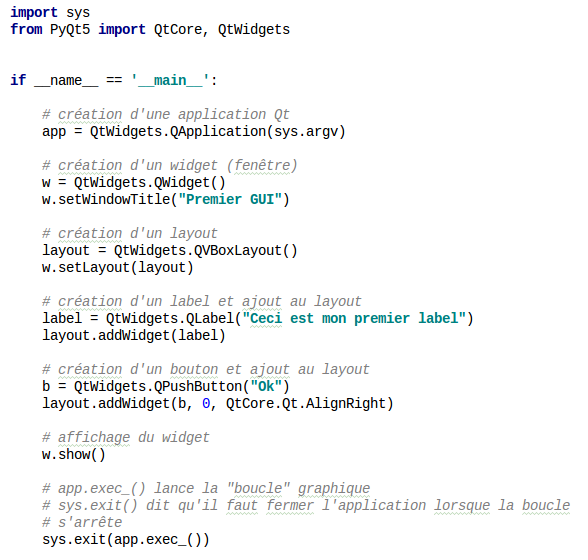
\includegraphics[width=0.7\textwidth]{img/widget0_1}\end{center}
\end{frame}

\begin{frame}[fragile]{\secname}{\subsecname}
\mytitle{Les éléments obligatoires}
\begin{itemize}
\item Le shebang (env et coding)
\item import du module sys
\item import du module QtWidgets de PyQt5: \\
\verb|from PyQt5 import QtWidgets|
\item Instanciation de la classe QApplication avec en argument sys.argv
\item sys.argv contient le chemin du script lancé et les éventuelles options passées au lancement du script
\item app.exec\_() lance une boucle d\rq{}écoute d\rq{}événements
\item sys.exit(app.exec\_()) termine le processus lorsque la boucle de l\rq{}application se termine
\end{itemize}
\end{frame}

% ~~~~~~~~~~~~~~~~~~~~~~~~~~~~~~~~~~~~~~~~~~~~~~~~~~~~~~~~~~~~~~~~~~~~~~~~~~~~~~
\subsection{Classe QApplication} 
\begin{frame}{\secname}{\subsecname}
\mytitle{QApplication}
\begin{itemize}
\item Doit être instanciée avant toute création d\rq{}objet graphique
\item Une seule instance pour l\rq{}application
\item Gère
\begin{itemize}
	\item l\rq{}ensemble des paramètres d\rq{}affichage de l\rq{}application
	\item les événements système et les envoie aux widgets (clic souris, touches clavier \dots)
	\item l\rq{}ensemble des éléments graphiques de l\rq{}application (qui a le focus, position de chaque éléments \ldots)
	\item l\rq{}internationalisation (langue système)
\end{itemize}
\end{itemize}
\end{frame}

% ~~~~~~~~~~~~~~~~~~~~~~~~~~~~~~~~~~~~~~~~~~~~~~~~~~~~~~~~~~~~~~~~~~~~~~~~~~~~~~
\subsection{Accesseurs et mutateurs}
\begin{frame}[fragile]{\secname}{\subsecname}
\begin{itemize}
\item accesseur: attribut()
\item mutateur: setAttribut(valeur)
\end{itemize}
\begin{center}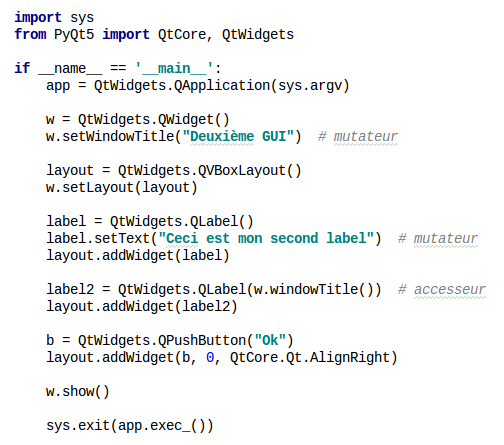
\includegraphics[height=0.7\textheight]{img/widget1_1}\end{center}
\end{frame}

%~~~~~~~~~~~~~~~~~~~~~~~~~~~~~~~~~~~~~~~~~~~~~~~~~~~~~~~~~~~~~~~~~~~~~~~~~~~~~~~
\subsection{Héritage}
\begin{frame}[fragile]{\secname}{\subsecname}
Pour créer et changer les attributs/méthodes d'un objet Qt il est plus simple de créer un objet qui hérite de cet objet
\begin{center}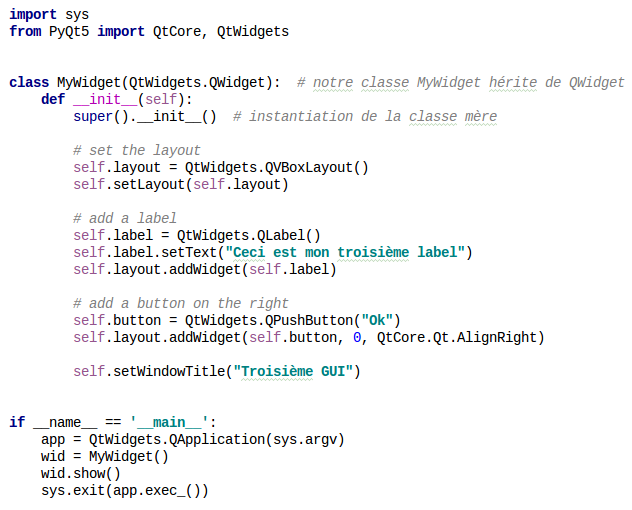
\includegraphics[height=0.7\textheight]{img/widget2_1}\end{center}
\end{frame}


% ==============================================================================
\section{Principaux éléments graphiques}

%~~~~~~~~~~~~~~~~~~~~~~~~~~~~~~~~~~~~~~~~~~~~~~~~~~~~~~~~~~~~~~~~~~~~~~~~~~~~~~~
\subsection{Layout}
\begin{frame}{\secname}{\subsecname}
Permet d\rq{}agencer les éléments graphiques (widgets) dans la fenêtre\\
~\\
\mytitle{QVBoxLayout: vertical, les widgets sont placés les uns sous les autres}
\begin{center}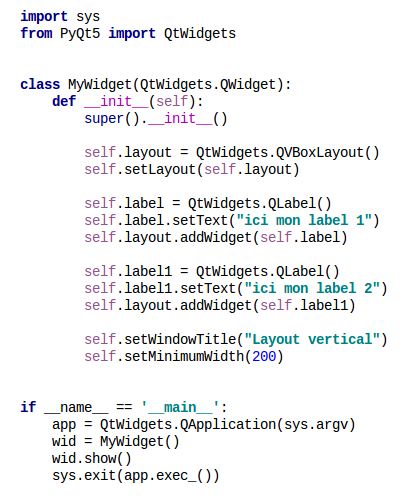
\includegraphics[scale=0.35]{img/widget3_1}\end{center}
\end{frame}

\begin{frame}{\secname}{\subsecname}
\mytitle{QHBoxLayout: horizontal, les widgets sont placés les uns à côté des autres}
\begin{center}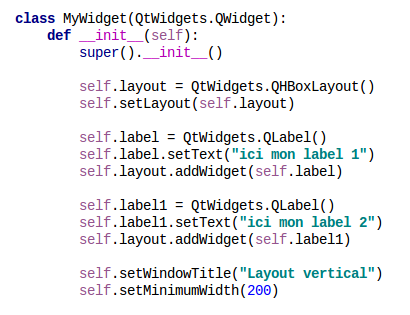
\includegraphics[scale=0.4]{img/widget4_1}\end{center}
\end{frame}

\begin{frame}{\secname}{\subsecname}
\mytitle{QFormLayout: pour créer un formulaire a 2 colonnes: label | widget}
\begin{center}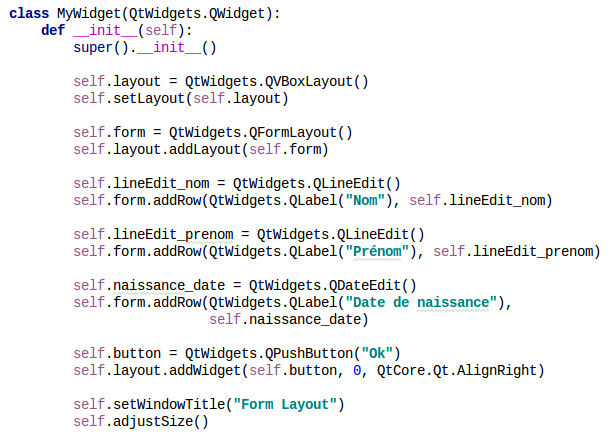
\includegraphics[scale=0.3]{img/widget5_1}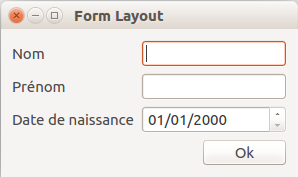
\includegraphics[scale=0.3]{img/widget5_1_fig}\end{center}
\end{frame}

\begin{frame}{\secname}{\subsecname}
\mytitle{QGridLayout: grille - Numérotation commence à 0, 0}
\begin{center}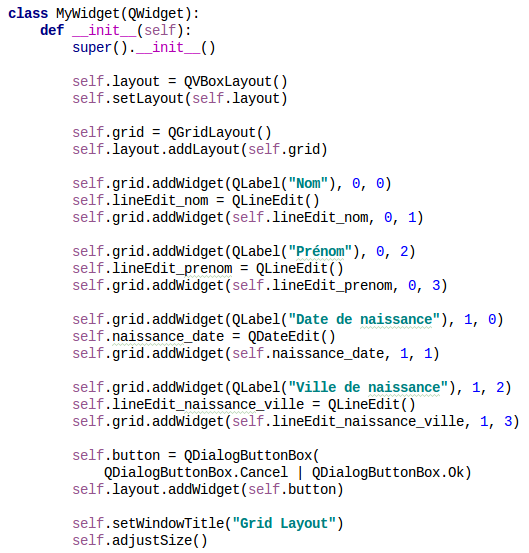
\includegraphics[scale=0.3]{img/widget6_1}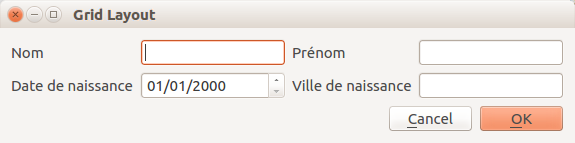
\includegraphics[scale=0.3]{img/widget6_1_fig}\end{center}
\end{frame}

%~~~~~~~~~~~~~~~~~~~~~~~~~~~~~~~~~~~~~~~~~~~~~~~~~~~~~~~~~~~~~~~~~~~~~~~~~~~~~~~
\subsection{Widgets}
\begin{frame}{\secname}{\subsecname}
Pour la documentation d\rq{}une classe: http://doc.qt.io/qt-5/nom\_classe\\
~\\
\begin{itemize}
\item QLabel: pour afficher du texte (\url{http://doc.qt.io/qt-5/qlabel.html})
\item QLineEdit: pour saisie de texte sur une ligne (\url{http://doc.qt.io/qt-5/qlineedit.html})
\item QTextEdit: pour saisie/affichage de texte sur plusieurs lignes (\url{http://doc.qt.io/qt-5/qtextedit.html})
\item QDialogButtonBox: boutons annuler et ok (\url{http://doc.qt.io/qt-5/qdialogbuttonbox.html})
\end{itemize}
\end{frame}

\begin{frame}{\secname}{\subsecname}
\mytitle{label, lineEdit, textEdit}
\begin{center}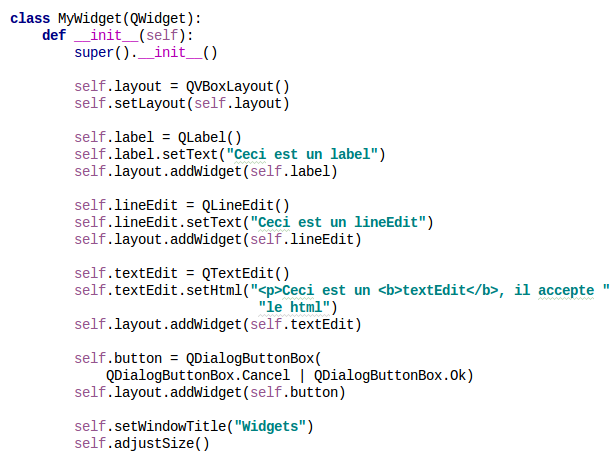
\includegraphics[scale=0.3]{img/widget7_1}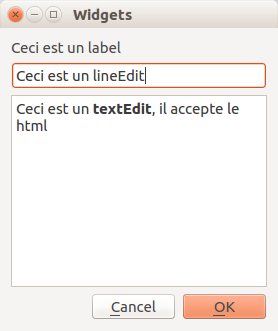
\includegraphics[scale=0.3]{img/widget7_1_fig}\end{center}
\end{frame}

\begin{frame}{\secname}{\subsecname}
\mytitle{QRadioButton: boutons radios}
\url{http://doc.qt.io/qt-5/qradiobutton.html}
\begin{center}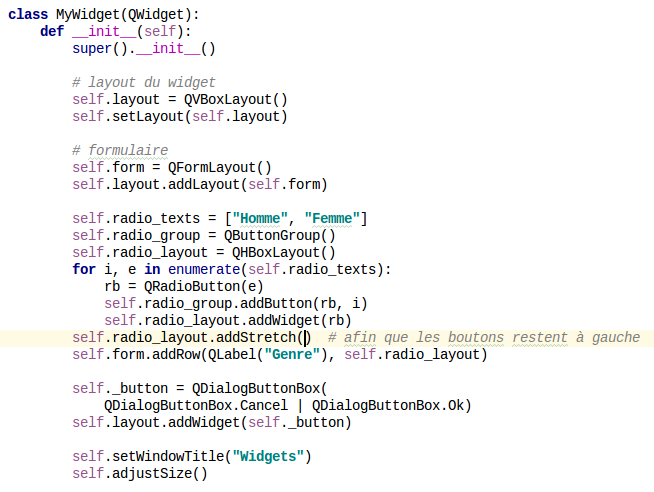
\includegraphics[scale=0.3]{img/widget8_1}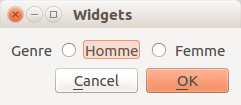
\includegraphics[scale=0.3]{img/widget8_1_fig}\end{center}
\end{frame}

\begin{frame}{\secname}{\subsecname}
\mytitle{QCheckbox: cases à cocher}
\url{http://doc.qt.io/qt-5/qcheckbox.html}
\begin{center}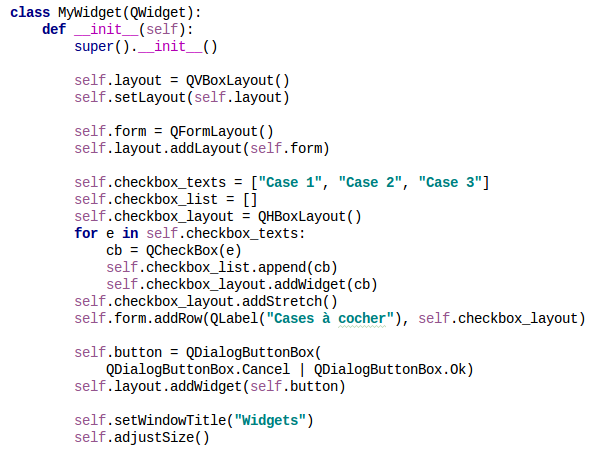
\includegraphics[scale=0.3]{img/widget9_1}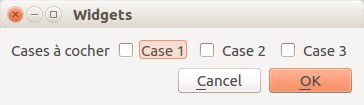
\includegraphics[scale=0.3]{img/widget9_1_fig}\end{center}
\end{frame}

\begin{frame}{\secname}{\subsecname}
\mytitle{QComboBox: liste déroulante}
\url{http://doc.qt.io/qt-5/qcombobox.html}
\begin{center}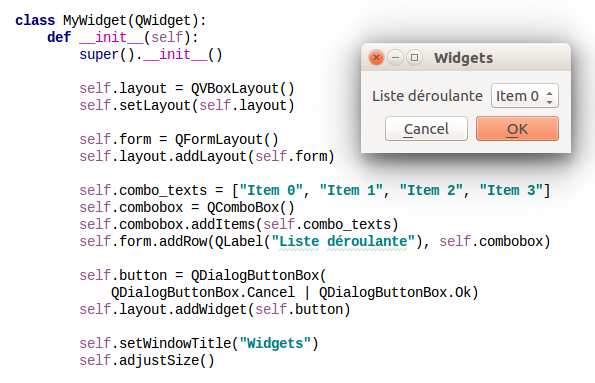
\includegraphics[scale=0.5]{img/widget10_1}\end{center}
\end{frame}

\begin{frame}[label=pratique1]{\secname}{\subsecname{} - Pratique}
Dans un fichier widget.py créer le widget suivant
\begin{center}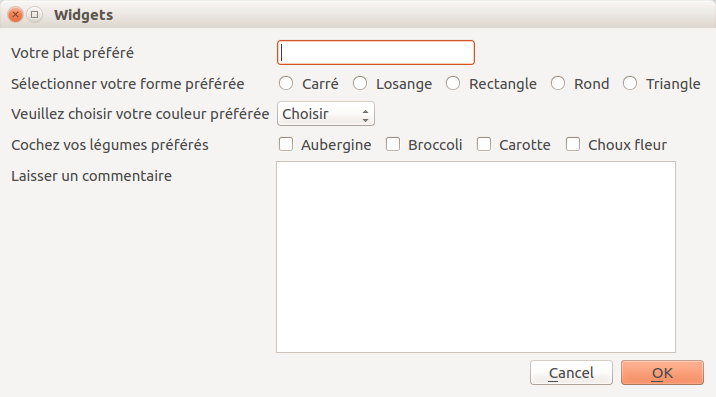
\includegraphics[scale=0.3]{img/widget_pratique_1_fig}\end{center}
\end{frame}

%~~~~~~~~~~~~~~~~~~~~~~~~~~~~~~~~~~~~~~~~~~~~~~~~~~~~~~~~~~~~~~~~~~~~~~~~~~~~~~~
\subsection{Windows}

\begin{frame}{\secname}{\subsecname}
\mytitle{QDialog}
\begin{itemize}
\item fenêtre modale (qui peut être attachée à une autre fenêtre)
\item peut fournir une valeur de retour (souvent accept/reject)
\item par défaut centrée sur sa fenêtre parente
%\item classe mère des boîtes de dialogue (cf. sous-section \href{boites_dialogue})
\end{itemize}
\begin{center}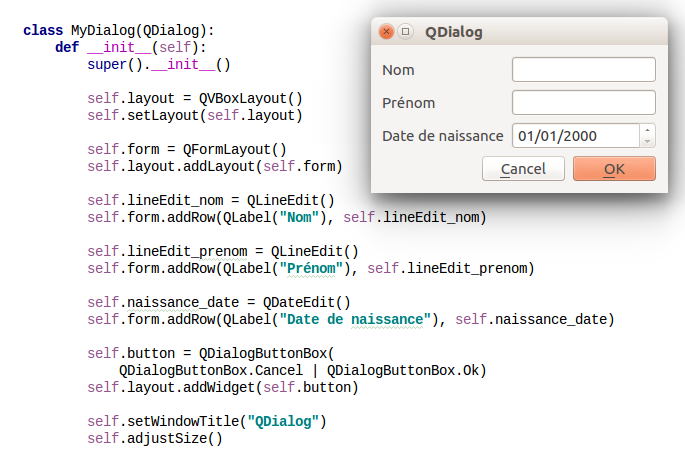
\includegraphics[scale=0.35]{img/window1_1}\end{center}
\end{frame}

\begin{frame}{\secname}{\subsecname}
\mytitle{QMainWindow}
\begin{itemize}
\item fenêtre principale d\rq{}une application
\item possibilité d\rq{}ajouter des menus
\end{itemize}
\begin{center}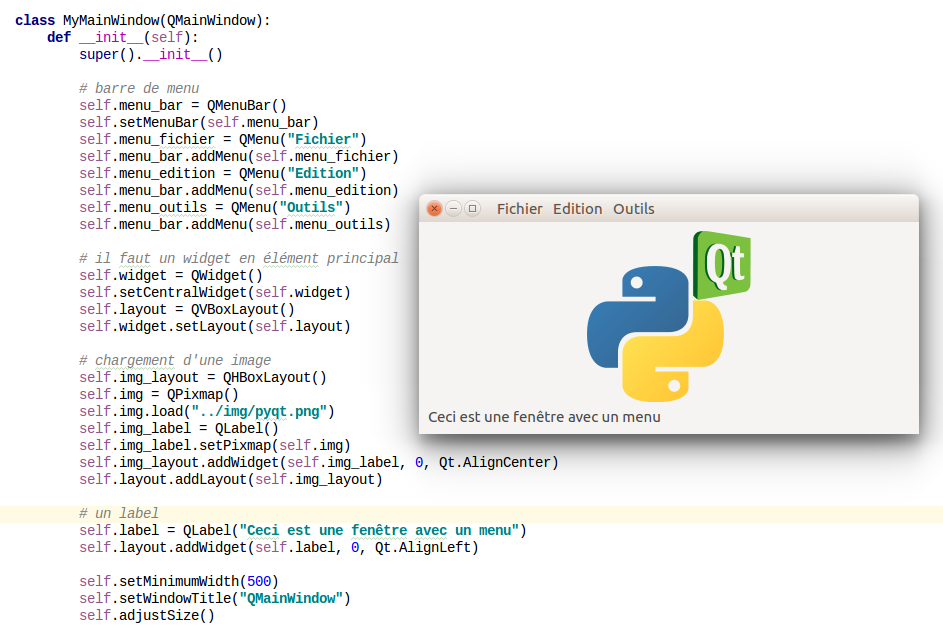
\includegraphics[scale=0.25]{img/window2_1}\end{center}
\end{frame}


%~~~~~~~~~~~~~~~~~~~~~~~~~~~~~~~~~~~~~~~~~~~~~~~~~~~~~~~~~~~~~~~~~~~~~~~~~~~~~~~
\subsection{Boîtes de dialogue\label{boites_dialogue}}

\begin{frame}{\secname}{\subsecname}
\mytitle{Information}
\begin{center}\includegraphics[scale=0.3]{img/boite1}\end{center}
~\\
\mytitle{Warning}
\begin{center}\includegraphics[scale=0.3]{img/boite2}\end{center}
\end{frame}

\begin{frame}{\secname}{\subsecname}
\mytitle{Critical}
\begin{center}\includegraphics[scale=0.3]{img/boite3}\end{center}
~\\
\mytitle{Question}
\begin{center}\includegraphics[scale=0.3]{img/boite4}\end{center}
\end{frame}

\begin{frame}{\secname}{\subsecname{}}
\mytitle{QFileDialog: Boîte de dialogue pour choisir un fichier ou un dossier}
\begin{itemize}
\item QtGui.QFileDialog.getExistingDirectory() pour choisir un dossier
\item QtGui.QFileDialog.getOpenFileName() pour choisir un fichier afin de l\rq{}ouvrir (mode lecture)
\item QtGui.QFileDialog.getSaveFileName() pour choisir un fichier afin d\rq{}enregistrer (création ou ouverture mode écriture)
\end{itemize}
\end{frame}

\begin{frame}{\secname}{\subsecname{}}
\mytitle{QFileDialog.getExistingDirectory}
\begin{center}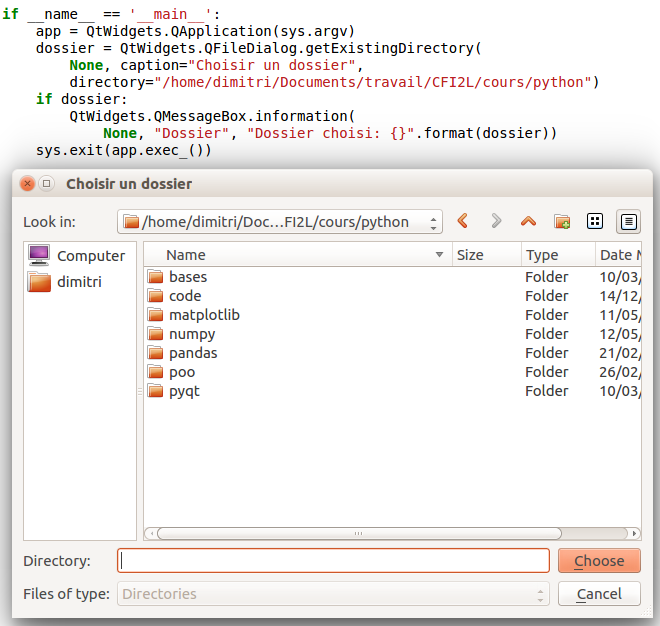
\includegraphics[scale=0.3]{img/filedialog1}\end{center}
\end{frame}

\begin{frame}{\secname}{\subsecname{}}
\mytitle{QFileDialog.getOpenFileName}
{\footnotesize filter=*.extension permet de filter l\rq{}affichage}
\begin{center}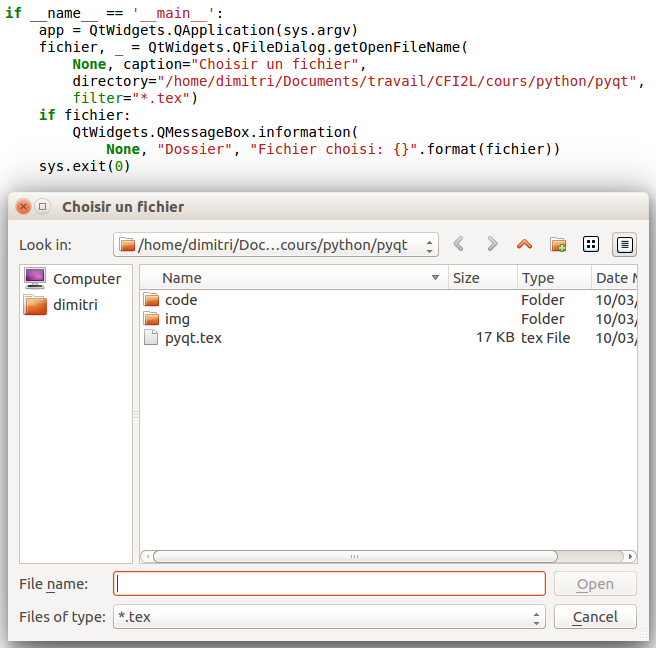
\includegraphics[scale=0.3]{img/filedialog2}\end{center}
\end{frame}

\begin{frame}{\secname}{\subsecname{}}
\mytitle{QFileDialog.getSaveFileName}
\begin{center}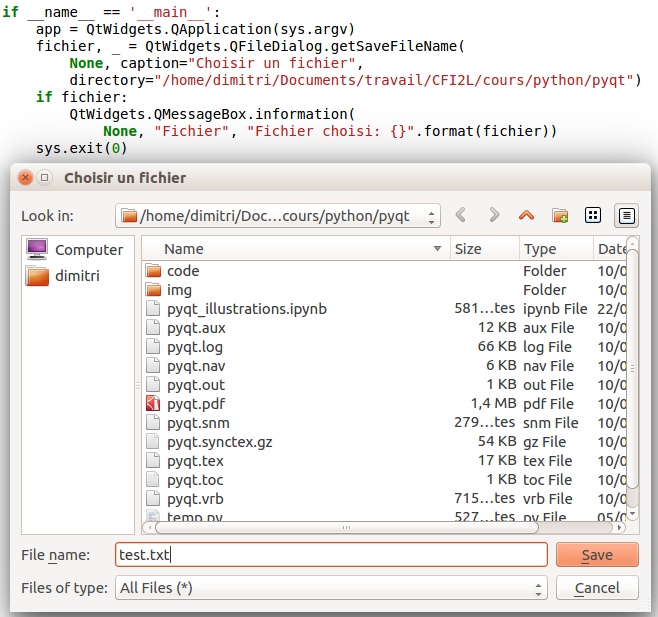
\includegraphics[scale=0.3]{img/filedialog3}\end{center}
\end{frame}


% ==============================================================================
\section{Gestion des événements} 

%~~~~~~~~~~~~~~~~~~~~~~~~~~~~~~~~~~~~~~~~~~~~~~~~~~~~~~~~~~~~~~~~~~~~~~~~~~~~~~~
\subsection{Fonctionnement} 
\begin{frame}{\secname}{\subsecname}
\mytitle{Signaux / Slots}
\begin{itemize}
\item Les objets émettent des signaux (clic sur un bouton, fermeture d\rq{}une fenêtre \ldots)
\item Les signaux peuvent être connectés à des slots (fonctions appelées en réponse au signal)
\item Ce mécanisme signaux/slots est très puissant et est une des caractéristiques de Qt
\item Pour connecter un signal à un slot utilisation de la fonction connect
\item Pour connaître les signaux émis par un objet Qt il faut regarder la documentation de Qt de l\rq{}objet dans la rubrique \lq\lq{}Signals\rq\rq{} (ou dans la classe mère de l\rq{}objet)
\end{itemize}
Exemple: Signaux émis par un pushbutton: \url{http://doc.qt.io/qt-5/qabstractbutton.html\#signals}
\end{frame}

\begin{frame}[fragile]{\secname}{\subsecname}
\mytitle{Click sur un bouton}
\begin{center}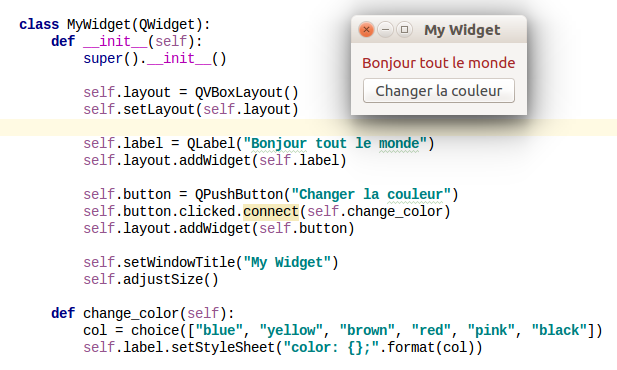
\includegraphics[scale=0.4]{img/signals1_1}\end{center}
\end{frame}

%~~~~~~~~~~~~~~~~~~~~~~~~~~~~~~~~~~~~~~~~~~~~~~~~~~~~~~~~~~~~~~~~~~~~~~~~~~~~~~~
\subsection{Signaux avec arguments}

\begin{frame}[fragile]{\secname}{\subsecname}
\mytitle{Si le signal envoie un argument (cf. définition du signal) et que l\rq{}on veut l\rq{}utiliser alors il faut que le slot/la fonction le déclare}
\begin{center}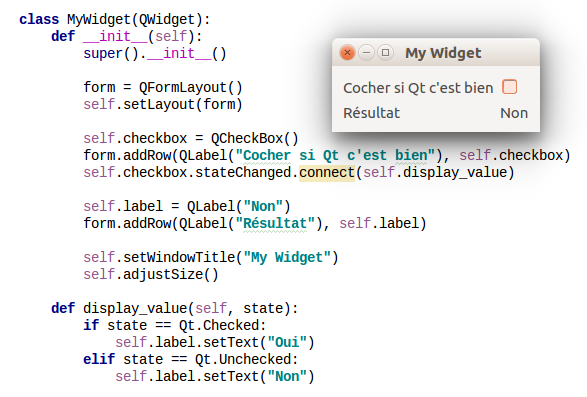
\includegraphics[scale=0.4]{img/signals2_1}\end{center}
\end{frame}

%~~~~~~~~~~~~~~~~~~~~~~~~~~~~~~~~~~~~~~~~~~~~~~~~~~~~~~~~~~~~~~~~~~~~~~~~~~~~~~~
\subsection{Principaux signaux}

\begin{frame}{\secname}{\subsecname}
\begin{itemize}
\item QAction (ajoutée à QMenu): triggered
\item QCheckBox: stateChanged(int state)
\item QDialogButtonBox: accepted (Ok), rejected (Cancel)
\item QLineEdit: textChanged(const QString \&text), editingFinished()
\item QPushButton, QRadioButton: clicked
\item QTextEdit: textChanged()
\item QComboBox: currentIndexChanged(int index)
\item \ldots
\end{itemize}
\end{frame}

\begin{frame}{\secname}{Pratique}
A partir de la fenêtre du slide \hyperlink{pratique1}{page \pageref{pratique1}}\\
(hériter de QDialog plutôt que de QWidget)\\~\\
\begin{itemize}
\item lorsque click sur cancel ou sur la croix, fermeture de l\rq{}application après confirmation (Quitter l\rq{}application?)
\item lorsque click sur ok, confirmation (Voulez-vous enregistrer les données saisies?)
\item si oui, vérification que tous les champs sont remplis
\item récupérer les textes, boutons sélectionnés etc.
\item afficher les données dans une boîte de dialogue
\end{itemize}
~\\
Aide: lorsque clic sur la croix, la fenêtre appelle la fonction reject. Il faut surcharger cette fonction.
\end{frame}


% ==============================================================================
\section{Qt Designer}

%~~~~~~~~~~~~~~~~~~~~~~~~~~~~~~~~~~~~~~~~~~~~~~~~~~~~~~~~~~~~~~~~~~~~~~~~~~~~~~~
\subsection{Présentation} 
\begin{frame}{\secname}{\subsecname}
\begin{itemize}
\item Outil fourni par Qt pour créer les interfaces graphiques en mode graphique
\item Permet de créer et placer facilement les widgets, d\rq{}éditer/modifier leurs attributs, de définir des connections signaux/slots, de gérer l\rq{}ordre des focus \ldots
\item Génère un fichier *.ui qu\rq{}il faut ensuite transformer en fichier python (*.py) grâce à la commande pyuic5 fichier.ui -o fichier.py
\end{itemize}
Documentation: \url{http://doc.qt.io/qt-5/qtdesigner-manual.html}
\end{frame}

%~~~~~~~~~~~~~~~~~~~~~~~~~~~~~~~~~~~~~~~~~~~~~~~~~~~~~~~~~~~~~~~~~~~~~~~~~~~~~~~
\subsection{Manipulation} 
\begin{frame}{\secname}{\subsecname}
\begin{itemize}
\item Création d\rq{}une fenêtre
\item Ajout de widgets (boutons, radiobutton, lineEdit, textEdit \ldots)
\item Placement des widgets dans la fenêtre (Horizontal/vertical layout, horizontal/vertical spacer \ldots)
\item Aperçu de la fenêtre
\item Edition / modification des attributs/propriétés des widgets
\item Edition des signaux/slots
\item Edition de l\rq{}ordre des tabulations
\item Conversion du fichier *.ui en *.py
\end{itemize}
\end{frame}

\begin{frame}{\secname}{\subsecname{} - Pratique}
Créer le widget suivant (à gauche en édition, à droite en prévisualisation)
\begin{center}\includegraphics[scale=0.3]{img/designer}\end{center}
\begin{itemize}
\item enregistrer le fichier 
\item le convertir en fichier *.py avec pyuic54
\end{itemize}
\end{frame}

\begin{frame}{\secname}{\subsecname{}}
\mytitle{Utilisation du fichier *.py dans un module}
\begin{itemize}
\item créer un module et faire un import du fichier py créé 
\item créer une classe qui hérite de QtGui.QDialog ou QtGui.QWidget selon
\item créer dans cette classe un objet qui instancie soit Ui\_Dialog soit Ui\_Form selon (QDialog ou QWidget)
\item appeler la méthode setupUi() de l'objet en passant self en argument
\item paramétrer les attributs de l'objet et définir les méthodes
\end{itemize}
\begin{center}\includegraphics[scale=0.3]{img/designer2}\end{center}
\end{frame}

%===============================================================================
%===============================================================================
%\begin{frame}{PyQt Pratique}{}
%\mytitle{Créer une application graphique de gestion de mots de passe}
%\end{frame}


%===============================================================================
\begin{frame}{Sources}
\begin{itemize}
\item \url{http://pyqt.sourceforge.net/Docs/PyQt4/}
\item \url{http://zetcode.com/gui/pyqt4/}
\item \href{http://openclassrooms.com/courses/programmez-avec-le-langage-c/introduction-a-qt}{Openclassroom}
\item \url{http://www.rkblog.rk.edu.pl/w/p/introduction-pyqt4/}
\end{itemize}
\end{frame}
\end{document}